\documentclass[border=10pt,margin=5pt,tikz,dvisvgm,rgb,utf8]{standalone}
\usepackage{ctex,xeCJK}  % 中文环境
\setCJKmainfont[BoldFont=Source Han Sans SC]{Source Han Serif SC}
\usepackage{calc,fontawesome,forest,smartdiagram,xcolor}
\usetikzlibrary{animations,arrows,automata,graphs,matrix,positioning,shadows,shapes}

\begin{document}
\renewcommand{\baselinestretch}{0.4}

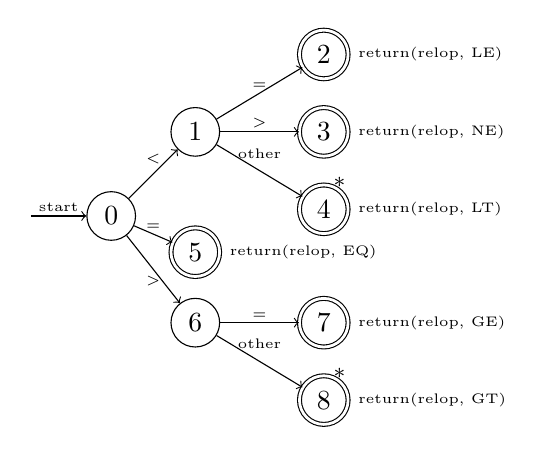
\begin{tikzpicture}
  \node[text width=-3em](start){};
  \node[circle, draw=black, right=2em of start](0){0};
  \node[circle, draw=black, above right=2.5em of 0](1){1};
  \node[circle, double, double distance=1pt, draw=black, right=of 1](3){3};
  \node[circle, double, double distance=1pt, draw=black, above=1em of 3](2){2};
  \node[circle, double, double distance=1pt, draw=black, below=1em of 3](4){4};
  \node[circle, double, double distance=1pt, draw=black, below=2.55em of 1](5){5};
  \node[circle, draw=black, below=0.75em of 5](6){6};
  \node[circle, double, double distance=1pt, draw=black, right=of 6](7){7};
  \node[circle, double, double distance=1pt, draw=black, below=1em of 7](8){8};

  \draw(start) edge[->] node[above=-2pt]{\tiny start} (0);
  \draw(0) edge[->] node[above=0pt]{\tiny <} (1);
  \draw(1) edge[->] node[above=-2pt]{\tiny =} (2);
  \draw(1) edge[->] node[above=-2pt]{\tiny >} (3);
  \draw(1) edge[->] node[above=1pt]{\tiny other} (4);
  \draw(0) edge[->] node[above=-2pt]{\tiny =} (5);
  \draw(0) edge[->] node[below=-1pt]{\tiny >} (6);
  \draw(6) edge[->] node[above=-2pt]{\tiny =} (7);
  \draw(6) edge[->] node[above=1pt]{\tiny other} (8);

  \node[right=0pt of 2](return2){\tiny return(relop, LE)};
  \node[right=0pt of 3](return3){\tiny return(relop, NE)};
  \draw[anchor=south west](4) node{\large ${}^{*}$};
  \node[right=0pt of 4](return4){\tiny return(relop, LT)};
  \node[right=0pt of 5](return5){\tiny return(relop, EQ)};
  \node[right=0pt of 7](return7){\tiny return(relop, GE)};
  \draw[anchor=south west](8) node{\large ${}^{*}$};
  \node[right=0pt of 8](return8){\tiny return(relop, GT)};
\end{tikzpicture}

\end{document}
